\documentclass{article}

% if you need to pass options to natbib, use, e.g.:
%     \PassOptionsToPackage{numbers, compress}{natbib}
% before loading neurips_2019

% ready for submission
% \usepackage{neurips_2019}

% to compile a preprint version, e.g., for submission to arXiv, add add the
% [preprint] option:
%     \usepackage[preprint]{neurips_2019}

% to compile a camera-ready version, add the [final] option, e.g.:
     \usepackage[final]{neurips_2019}

% to avoid loading the natbib package, add option nonatbib:
%     \usepackage[nonatbib]{neurips_2019}
\usepackage{float}          % to allow floating figures (ie placement in text)
\usepackage[utf8]{inputenc} % allow utf-8 input
\usepackage[T1]{fontenc}    % use 8-bit T1 fonts
\usepackage{hyperref}       % hyperlinks
\usepackage{url}            % simple URL typesetting
% \usepackage{booktabs}       % professional-quality tables
\usepackage{amsfonts}       % blackboard math symbols
% \usepackage{nicefrac}       % compact symbols for 1/2, etc.
% \usepackage{microtype}      % microtypography
% Others added after
\usepackage{breqn}          % break equations over multiple lines
% \usepackage{cite}           % citing references
% \usepackage{biblatex}
\usepackage{graphicx}       % for images
\usepackage{soul}           % highlight text
\usepackage{xcolor}          % highlight in math
\newcommand{\mathcolorbox}[2]{\colorbox{#1}{$\displaystyle #2$}}
\usepackage[section]{placeins} % for overflow on text after figures
\def\BibTeX{{\rm B\kern-.05em{\sc i\kern-.025em b}\kern-.08em
    T\kern-.1667em\lower.7ex\hbox{E}\kern-.125emX}}

% \usepackage[
%   backend=biber,
%   style=alphabetic,
%   sorting=ynt
%   ]{biblatex}
%   \addbibresource{sample.bib}

\usepackage{amsmath}        % for text in math equations
\graphicspath{ {./images/}}

\title{Multiagent Reinforcement Learning in a Synchronous Strategy Game}

\author{%
  Ahmed Siddiqui \\
  Faculty of Computer Science\\
  University of Victoria\\
  Victoria, CA V8P 5C2 \\
  \texttt{jesuisahmedn@gmail.com } \\
  \And
  Louis Kraak  \\
  Faculty of Engineering \\
  University of Victoria \\
  Victoria, CA V8P 5C2 \\
  \texttt{lkraak@uvic.ca} \\
  \And
  Michail Roesli  \\
  Faculty of Engineering \\
  University of Victoria \\
  Victoria, CA V8P 5C2 \\
  \texttt{mroesli@uvic.ca} \\
  \And
  Swapnil Daxini  \\
  Faculty of Physics and Astronomy \\
  University of Victoria \\
  Victoria, CA V8P 5C2 \\
  \texttt{swapneel.dx8@gmail.com} \\
  \And
  Yang Li  \\
  Faculty of Computer Science \\
  University of Victoria \\
  Victoria, CA V8P 5C2 \\
  \texttt{leo19970804@gmail.com } \\
}

\DeclareMathOperator*{\argmax}{arg\,max}
\DeclareMathOperator*{\argmin}{arg\,min}

\begin{document}

\maketitle

\begin{abstract}
  A lot of studies have been done on reinforcement learning recently. Q
  learning, or DQN tries to solve the single agent vs environment problem, where
  some other approaches such as AlphaGo attempt the double agent game. In this
  project, we try to find an algorithm to generate an agent that performs well
  in a multiagent synchronous strategy game.
\end{abstract}

\section{Introduction}

Battlesnake is a synchronous strategy game. It is simply a multiplayer version
of the classic game Snake. The version we are training with is a 11x11 game
board with 4 snakes. In each round, players choose an action from the space
\textit{left,right,up,down}, the snake's head and body will then move accordingly. If
a snake's head runs into any obstacle (a snake's body or wall), it dies. If it
runs into another snake's head, the shorter snake dies (in a tied situation both
snakes die). If it runs into a food, its length will grow by 1, and its health
point resets to 100. Every turn, all snake's health will decrease by 1, and once
it reaches 0 the snake dies. The last snake alive becomes the winner of the
game. If no snakes live, it is considered a draw. See the reference for a more
detailed description \cite{BattlesnakeDoc}. An image of such a game is shown
below in figure \ref{fig:snake}.

% Figure Here

\begin{figure}[!ht]
  \centering
  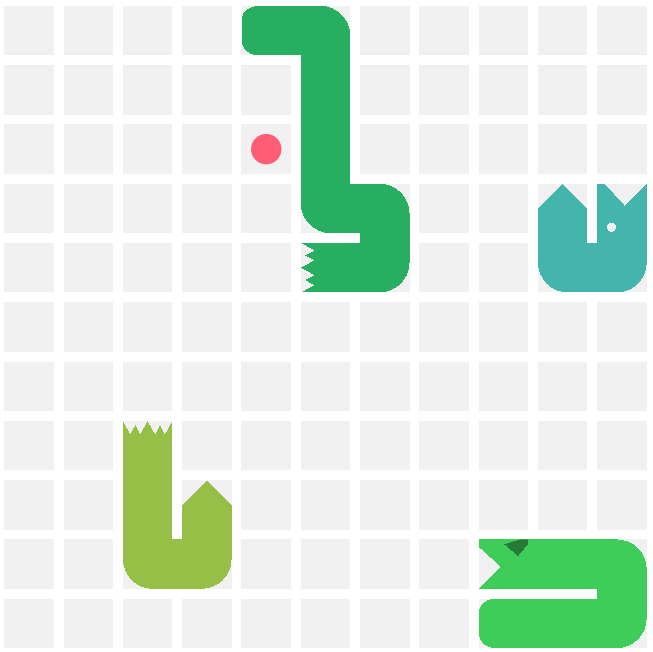
\includegraphics[width=6cm]{snake}
  \caption{A game of battlesnake in-progress.}
  \label{fig:snake}
\end{figure}

\section{Related Work}

AlphaSnake Zero uses the same approach that AlphaGo Zero used
\cite{AlphaGoZeroPaper}, where the training algorithm consists of 3 stages,
self-play, training and pit. Due to the lack of a powerful computing device (a
TPU), the network for AlphaSnake is simplified. AlphaGo uses a two headed
network to compute the value (roughly interpreted as win rate) of the current
game board, and also a policy to guide the next action. As this is a
reinforcement learning problem, there is no true label that we can assign to the
training data. Instead, a Monte Carlo Tree Search is used to get a good
estimate of the optimal policy. See figure \ref{fig:mcts} to see the steps of
the Monte Carlo tree search algorithm.

\begin{figure}[!ht]
  \centering
  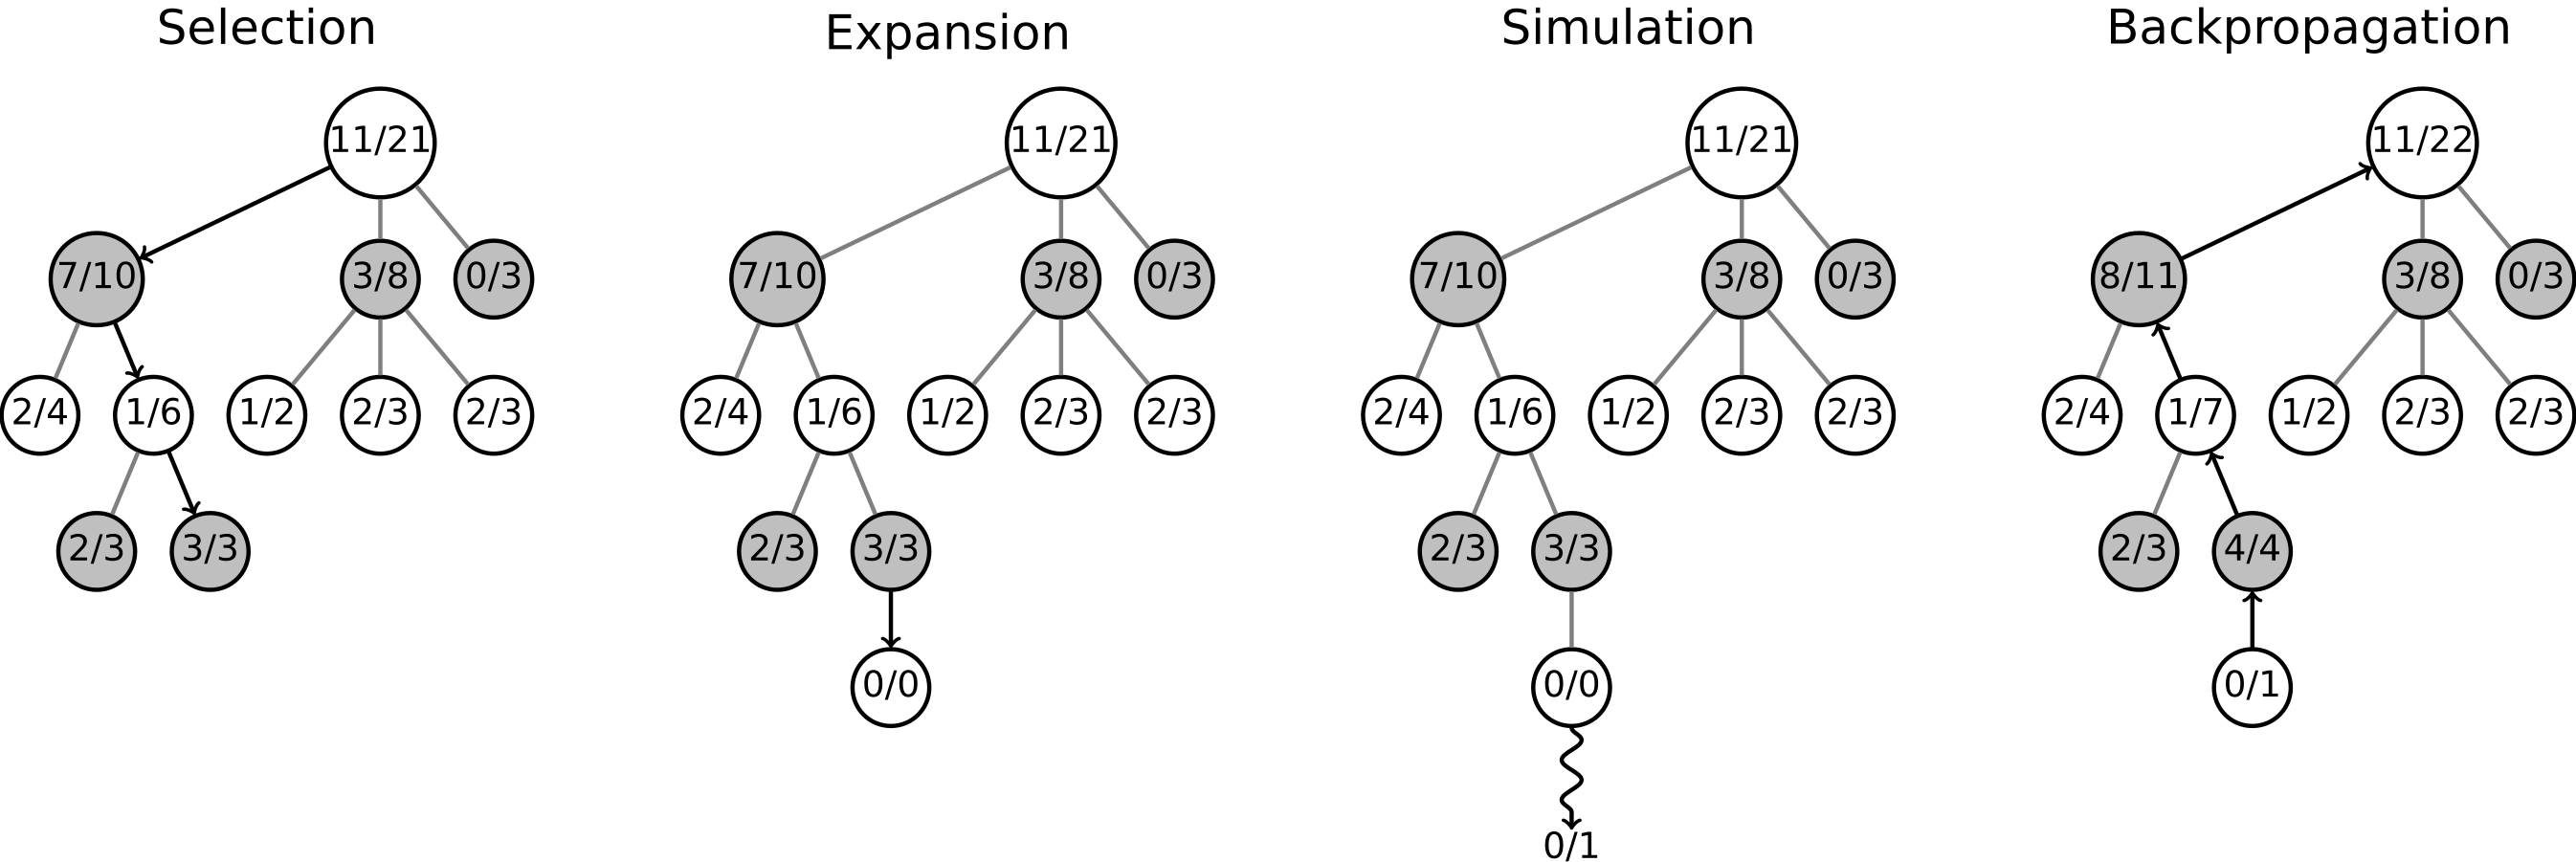
\includegraphics[width=12cm]{MCTS}
  \caption{Steps of the MCTS algorithm}
  \label{fig:mcts}
\end{figure}

\FloatBarrier

\section{Method}

In each iteration, a number of games are played using the current neural
network, with data being recorded for training. For each turn of the game, we
keep the information of the game board (the state), the move each snake made
(the action), the computed Q values (estimated win rate), the transition
probability (explained later). Then we use the data to train the network. After
training, the new network competes against the old one and further replace it if
performance is better. A general overview of this AI is shown in figure
\ref{fig:overview_of_model} below. CNN stands for convolutional neural network.
The CNN takes as input a state representing the game from a player's point of
view, and computes as output the Q values of each action. Then a policy (a
probability distribution of all actions) is computed to guide the AI.

\begin{figure}[!ht]
  \centering
  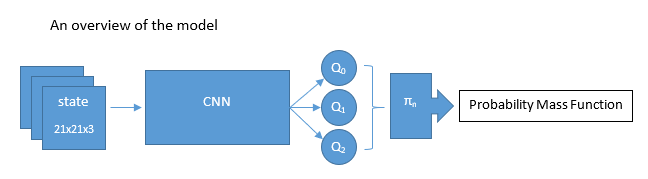
\includegraphics[width=\linewidth]{overview_of_model}
  \caption{AlphaSnake Zero Model}
  \label{fig:overview_of_model}
\end{figure}

\FloatBarrier

For the input of the network, we need something that can recover enough
information of the game board. The designed state representation is as
follows: The state is a 21x21x3 tensor. The game board is only 11x11, but the
network will quickly struggle to identify where its own head lies. To combat this,
the view of the game is centered at the snake's head, allowing immediate
recognition of relative position. Imagine you are the snake and you view the
world around you, so a 21x21 board is needed to percieve the original board in
the worst case (if we are at the edge). Additionally, every snake has
its own view of the board. The objects in the game are also classified into
three channels explained below.

There are essentially three fundamental things in the game: things that if you run into you
die (body and wall); if you run into, you grow (food); and if you run into
some snake, you die (head). Thus, the game board is classified into 3
channels. The first layer is the picture of all the snakes' heads. The second
one is for all the 'deadly' obstacles (bodies and walls). And the last one shows
all the food on the board. In all layers, 0 means an empty cell.

In the first layer, the value of a snake's head is the snake's length relative
to the current player, so a negative value means a shorter snake's head and vice
versa. Since a snake of the same length as you also kills you, the value of its
head is also negative. Overall, the value roughly tells you how dangerous a
block is. The formula for computing the head value is simply

\begin{equation}
  value = (\text{length of the snake}-\text{length of you}+0.5) \times \text{multiplier}
\end{equation}

where the multiplier is to keep the value in the range of [-1, 1] for training
purposes. The 0.5 solves two problems, one mentioned earlier about the snake of
same length, and it avoids the value inside the brackets being zero, causing an
'invisible head'.

In the second layer, the wall is simply represented with 1. We also need
something to recover the direction of a body bock, since it holds the
information about how the snake moves on the board. But what is really essential
is how long a body block will remain at its position. If we represent the body
as the number of turns until it will be away, then we can roughly recover the
information of a snake by tracing the increasing value of the body blocks. The
number of turns until it will be removed is simply the body length measured from
that body block to the tail of the snake. The value is calculated using the
following formula

\begin{equation}
  value = (\text{number of turns until it's removed}) \times \text{multiplier}
\end{equation}

There are degenerate cases where it is not possible to tell which body belongs
to which snake, but body blocks all work the same way, so it does not matter.

In the last layer, all the food is labeled according to the snake's health points. This
has a huge benefit to reducing the difficulty of learning. It strongly relates
the food to health, and no explicit information for health needs to be
stored.

\begin{equation}
  value = (101-\text{your health}) \times \text{multiplier}
\end{equation}

Note that for this representation of states, it is impossible to recover the health of other snakes, but
according to the experience of Battlesnake tournaments, it is not a useful
information, as death due to starvation almost never happens in high level
games. We use 101 instead of 100 to avoid the value inside the brackets being
zero, resulting in 'invisible food'.

For the output of the network, we need something that can guide the action to
take. A policy could be a good choice, but unlike the game of Go, where a move
usually just adds another piece on the board, MCTS is too expensive for
Battlesnake, because a move will drastically change the game board and thus be very
slow to compute. Instead of approximating the optimal policy, it is easier to
obtain a good estimation of the Q values. Assume the optimal function for Q
value is $Q(s,a)$, where it takes as input the current state $s$ and the action
$a$, and it outputs the value (win rate) of the player if that action $a$ is
chosen under state $s$. An obvious fact is that a game board of Battlesnake is
equivalent to its rotation and reflections (with actions also rotated or
reflected, of course). Thus, we can rotate the board so that the snake is always
facing upwards. This mainly has two benefits. First, it automatically treats all
rotations as one, thus reducing overfitting. Second, there is always a backward
move that immediately kills you (run into your own body), so this action is
meaningless to evaluate. If the snake is always facing up, the output space can
be transformed into \textit{turn left,go straight,turn right}, represented by
numeric values {0,1,2}. It simplifies the network and training. Although it is
true that only for the very first move, there are technically four choices, but
we don't care about that one move so much that we want to expand the output
space. During the training, we can also make the reflections of the board and Q
value vectors to force the network to realize symmetry, and hopefully reduce
overfitting. Once we have the 3 dimensional vector $\langle Q(s,0),Q(s,1),Q(s,2)
  \rangle$, namely the Q value of each action $a_i$ given the current state s, a
softmax-like function is going to generate a probability mass function based on
the values, which is the policy. The softmax-like function, denoted $\pi$, is simply
softmax with exponent n instead of e.

\begin{equation}
  \pi_n(\overrightarrow{v})=\overrightarrow{v}^{\circ n}\cdot(\sum\limits_i \overrightarrow{v}^{\circ n}i)^{-1}
\end{equation}

Here, $\overrightarrow{v}$ is a vector and $n$ is a constant.
$\overrightarrow{v}^{\circ n}$ denotes the element-wise power. By picking
the n, we can control how explorative the snake is, the higher n is, the
more it highlights the higher values in $\overrightarrow{v}$, and thus it
would not bother to pick the lower valued actions.

To get a good estimate of the value function without MCTS, we label the Q values
according to the following criteria. From the point of view of any snake, the
transition between states is not deterministic. The transition is a Markov
process because it depends on how other snake moves. Let the function
$\Psi(s_0,a,s_1)$ represents the probability of entering state $s_1$, if you
take the action a at current state $s_0$. Let the Q value vector of state $s_0$
be $\langle Q(s_0,0),Q(s_0,1),Q(s_0,2) \rangle$. Say $Q(s_0,a)$ is high and you
pick this action a. Now with probability $\Psi(s_0,a,s_1)$, we then have entered
the next state $s_1$, and we now get the Q values $\langle
  Q(s_1,0),Q(s_1,1),Q(s_1,2) \rangle$. Since the Q values represent win rate, the
optimal strategy is to pick $\argmax_{a_i}Q(s_1,a_i)$. Then we can say that, at
state $s_0$, if we pick action a, with probability $\Psi(s_0,a,s_1)$, we end up
with a win rate of $\max_{a_i}Q(s_1,a_i)$. Obviously, we can see that the Q
value is a weighted sum of the max Q values of its successor states, thus we
have

\begin{equation}
  Q(s_0, a) = \sum\limits_{s_i}\Psi(s_0,a,s_i)\max_{a_j} Q(s_i,a_j)
\end{equation}

This equation is the core part of AlphaSnake Zero's training algorithm. We can
now refine the Q value vector by updating its explored entry $Q(s_0,a)$. A
complete record of a game play gives a chain of states for each snake. We update
the Q values recursively, from the very last state to the first. We know what
$\max_{a_i}Q(s_1,a_i)$ is, namely the max value of the successor of $s_0$ recorded
in the chain of states. Assuming the network is already somewhat accurate, we
don't want to change $Q(s_0,a)$ unless $\max_{a_i}Q(s_1,a_i)$ has been refined. If
$\max_{a_i}Q(s_1,a_i)$ was updated to $\max_{a_i}Q^*(s_1,a_i)$ during the
previous step, then we want the new $Q^*(s_0,a)$ to be

\begin{dmath}
  \Psi(s_0,a,s_1) \times \max_{a_i}Q^*(s_1,a_i) + \sum\limits_{s_i\neq
    s_1}\Psi(s_0,a,s_i)\max_{a_j}Q(s_i,a_j) =
  \Psi(s_0,a,s_1)\times\max_{a_i}Q^*(s_1,a_i) +
  \sum\limits_{s_i} \Psi(s_0,a,s_i)\max_{a_j}Q(s_i,a_j)
  - \Psi(s_0,a,s_1) \times \max_{a_i}Q(s_1,a) =
  \Psi(s_0,a,s_1) \times [\max_{a_i}Q^*(s_1,a_i) -
    \max_{a_i}Q(s_1,a_i)]+\sum\limits_{s_i}
  \Psi(s_0,a,s_i)\max_{a_j}Q(s_i,a_j) = \Psi(s_0,a,s_1) \times
  [\max_{a_i}Q^*(s_1,a_i) - \max_{a_i}Q(s_1,a_i)] +
  Q(s_0,a)
\end{dmath}

We can see that if the max of its successor was unchanged then the new value
$Q^*(s_0,a)$ just remains unchanged, too. There is, however, a flaw in this
updating method. It has no guarantee on that the new Q value staying in the
range [0, 1], which is the practical range for win rate, and also the range for
the sigmoid function. In practice, if the network is already somewhat good, a
bad value should almost never happen, but we are still supposed to set the bound
manually. If it does happen, say the new $Q^*(s_0,a)\geq 1$, then this one is
guaranteed to be the new maximum since all other Q values is computed by sigmoid
and thus less than 1. Then, it very likely will shoot up its parent state's Q
value over 1 and recursively messes up the whole chain of states. Thus, we
assign the following bounded value to $Q^*(s_0,a)$.

\begin{equation}
  min(max(\Psi(s_0,a,s_1)\times [\max_{a_i}Q^*(s_1,a_i)-\max_{a_i}Q(s_1,a_i)]+Q(s_0,a),0),1)
\end{equation}

To complete the final piece of our estimation of Q values, we need to know
$\Psi$, the transition probability. If we get the actions of every snake, then
the transition is almost deterministic, except the food spawns randomly, but
that is a minor factor. Obviously, since the game is synchronous, the
probability of any snake taking an action is independent from others.
$\Psi(s_0,a,s_1)$ is almost equal to the product of some entry of each policy
calculated by other snakes. Let the transition function
$\Gamma(s,\overrightarrow{A})$ computes the successor state of $s$ given
$\overrightarrow{A}$, a vector of actions of snakes (omitting the randomness of
food).

\begin{equation}
  \Psi(s_o,a,\Gamma(s_o,\langle a, a_1, \ldots , a_k \rangle )) \approx \Pi^k_{i=1}\pi_n{(\langle Q(s_i,0),Q(s_i,1),Q(s_i,2) \rangle)}_{a_i}
\end{equation}

Here $\pi_n$ is the softmax-like function, $s_i$ is the ith snake's view of
state $s_0$ (not including you since you explicitly made action a), and $a_i
  \in {0,1,2}$ is the action it chose. There is one exception; if a snake made
an action and died right after, then the assigned value is simply 0 since it
is usually not relevant to what last moves other snakes chose unless it died
due to head on head collision.

Since the training data is massive, a good trick is to obtain a sample from the
training data. There are various ways to sample the data, but one thing to
realize is that late game might be far more important than the early game. The
sampling method used in the training algorithm makes an exponentially growing
gap between samples counting from the last move, to the first. Another trick
is to use batch normalization between layers in the network because
reinforcement learning tends to change the input distribution, it introduces
instability to the learning, and batch normalization can address that problem.
Another problem we encountered during training is that after some number of
iterations, the snakes realize that if it runs into something they die, so they
come up with the so-called 'chicken snake' strategy, where one snake just
moves in circles and does nothing. In other words, it is stuck at a local optimum.
To avoid this, we let the snake learn in a modified environment where every turn
the health is reduced by 9, so it will quickly die from starvation and force it
to go look for food. After that, we put it into the original environment. We
call that 'learn to walk before you run'. Be careful with the choice of the
decrement value. We still want it to realize that once the health gets to 1, it
will die next turn, so the decrement must be a factor of 99. If we prime
factorize 99, we can see the only options are 1, 3, 9, 11, 33, 99.

After training, the newly trained network is to be compared with the old network.
Several games are played between them (can use different competing rules,
1v3 or 2v2, etc.). If the new network's win rate surpasses a threshold, it will
replace the old one. A good way to select the threshold is to use a binomial
distribution to figure out a value such that a worse network (say a win rate
less than 50\% in 2v2 games) has a negligible chance of surpassing it.


\section{Experiments and Discussion}

With limited computational power, we tried the algorithm on a small CNN. It
consists of 6 convolutional hidden layers, with 32, 32, 64, 64, 128, 128 filters
of size 3x3, respectively. It used 'selu' as activation function
\cite{SeluPaper}, and batch normalization layers are added between the weights
and activation functions. After running for 154 iterations, we obtained the
following results as seen in figure \ref{fig:cause_of_death} and figure
\ref{fig:average_food_eaten} below.

\begin{figure}[!ht]
  \centering
  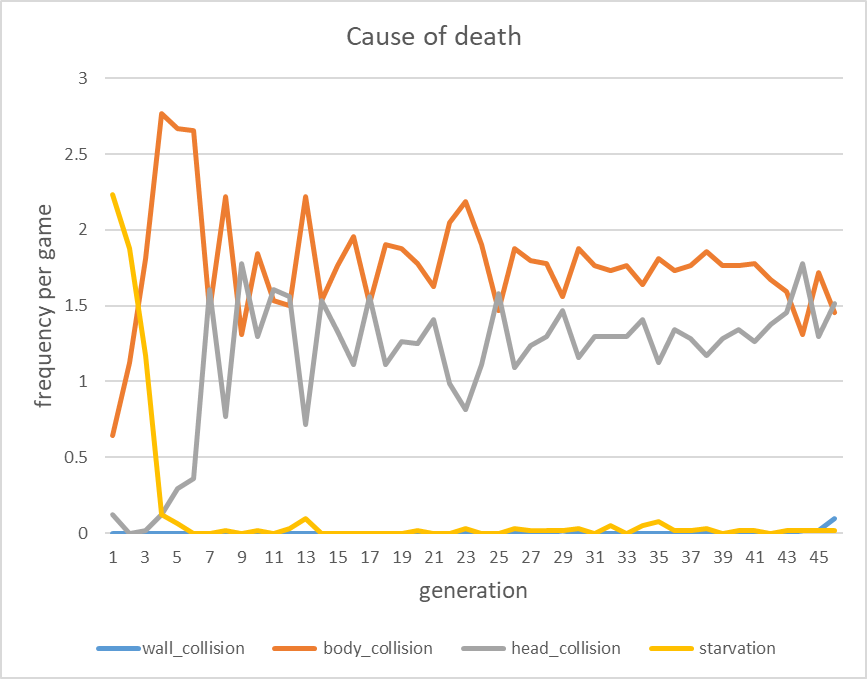
\includegraphics[width=300px]{cause_of_death}
  \caption{Cause of Death}
  \label{fig:cause_of_death}
\end{figure}

\FloatBarrier

Figure \ref{fig:cause_of_death} above, further analyses the cause of death for
the first 45 generations. The algorithm quickly learns the basics of the game as
the deaths by starvation and wall collisions are close to zero following the 6th
generation.  However, interestingly, the number of deaths by head collisions is
quite high.  This is likely due to the algorithm not being able to control its
aggressiveness between smaller and larger snakes.

\begin{figure}[!ht]
  \centering
  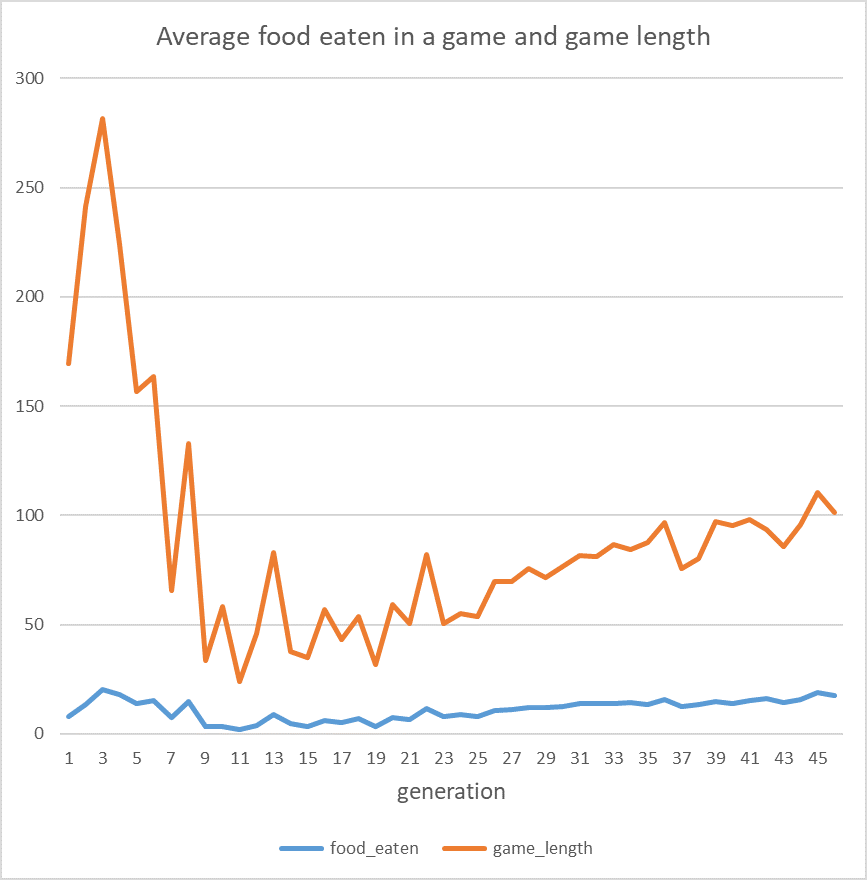
\includegraphics[width=300px]{average_food_eaten}
  \caption{Average Food Eaten}
  \label{fig:average_food_eaten}
\end{figure}

\FloatBarrier

Figure \ref{fig:average_food_eaten} above depicts the average food eaten per
game as well as the game length. We see an upward trend on the game length,
suggesting that further training would result in an overall smarter AI for
the snake.

Other experiments that we have conducted were to compare 16 different
generations against the best training snake provided by the battlesnake team. We
compared the winrate, the average time steps in a game, the average food eaten
in a game, the average number of collisions in a game, and the average number of
heads hunted in a game in figure \ref{fig:winrate}, \ref{fig:time_steps},
\ref{fig:food_eaten}, \ref{fig:collisions}, \ref{fig:heads_hunted} respectively.
Generally, we noticed that as the number of model generations/ training
iterations increased the winrate, average time steps, food eaten, and heads
hunted increased, while the average number of collisions decreased which are all
consistent with what we'd predict with the increasing winrate as it is getting a
better understanding of the rules of the game.

\begin{figure}[!ht]
  \centering
  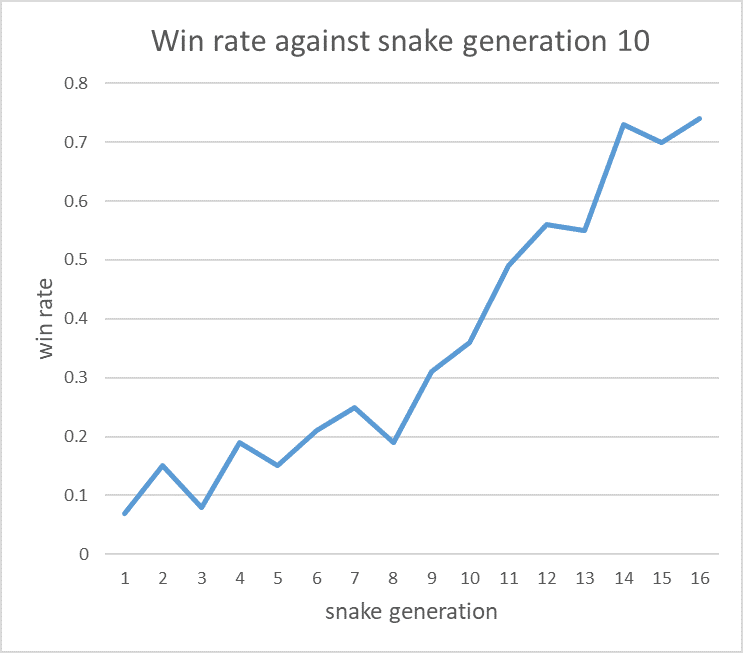
\includegraphics[width=300px]{winrate}
  \caption{Winrate}
  \label{fig:winrate}
\end{figure}
\FloatBarrier

\begin{figure}[!ht]
  \centering
  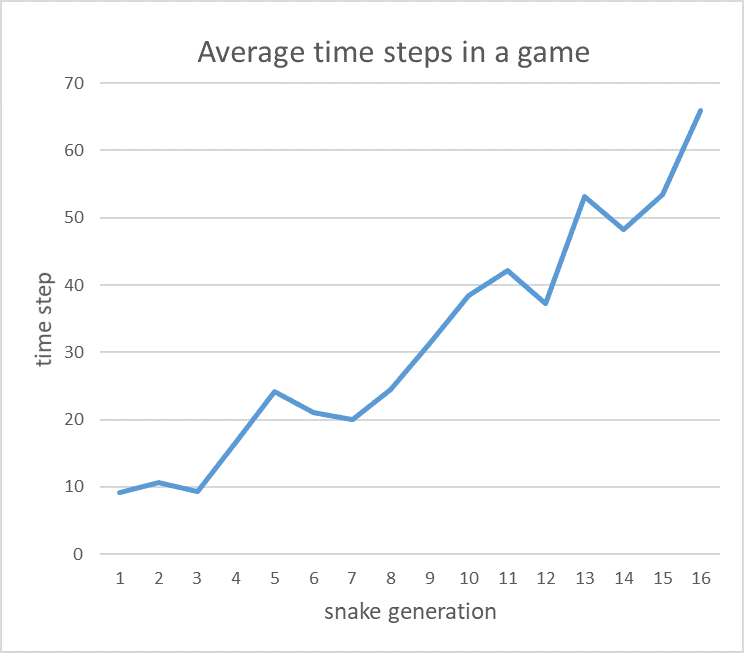
\includegraphics[width=300px]{time_steps}
  \caption{Average Number of Time Steps}
  \label{fig:time_steps}
\end{figure}
\FloatBarrier

\begin{figure}[!ht]
  \centering
  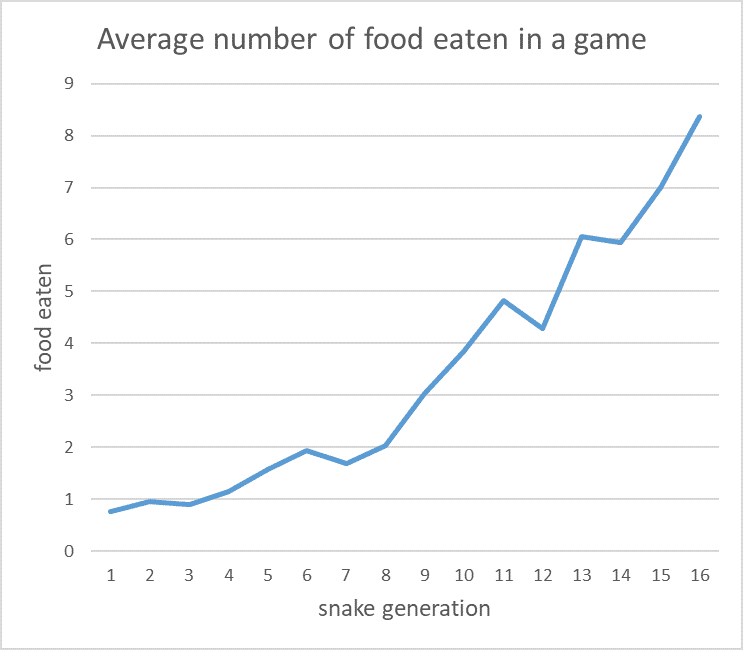
\includegraphics[width=300px]{food_eaten}
  \caption{Average Number of Food Eaten}
  \label{fig:food_eaten}
\end{figure}
\FloatBarrier

\begin{figure}[!ht]
  \centering
  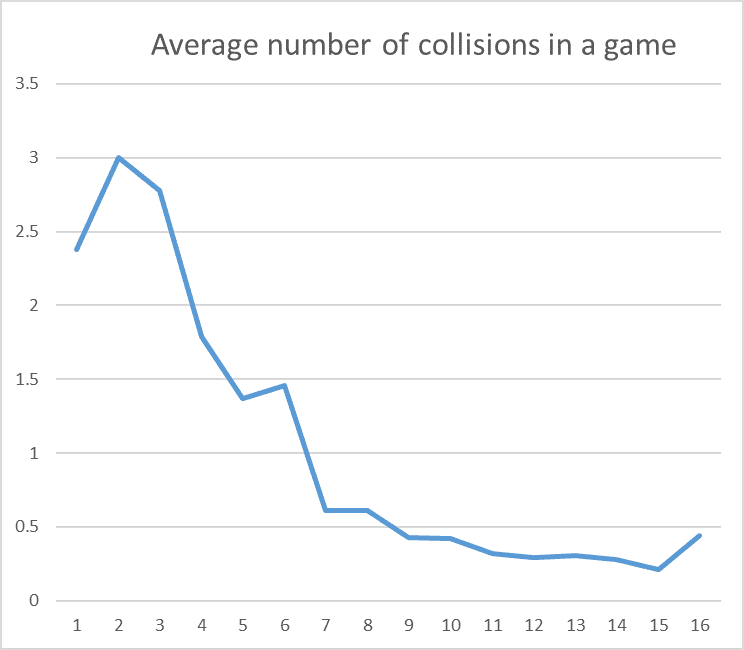
\includegraphics[width=300px]{collisions}
  \caption{Average Number of Collisions}
  \label{fig:collisions}
\end{figure}
\FloatBarrier

\begin{figure}[!ht]
  \centering
  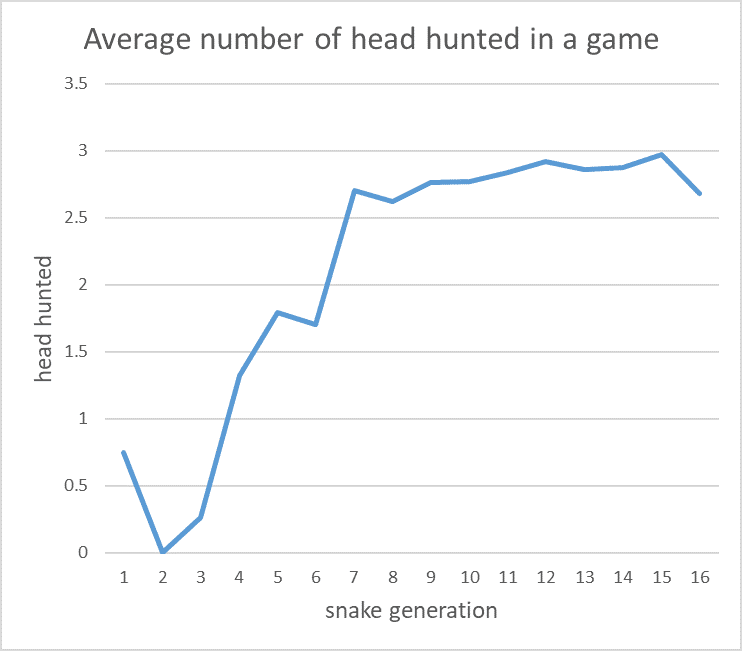
\includegraphics[width=275px]{heads_hunted}
  \caption{Average Number of Heads Hunted}
  \label{fig:heads_hunted}
\end{figure}
\FloatBarrier

For the final experiment, three different generations of the snakes were added
to the Battlesnake arena to compete against other snake AIs. All performed quite
well and currently in the top 150 of the leaderboard. The 10th and 15th
generation AlphaSnake Zero currently sits at 147th and 135th position on the
leaderboards respectively. The 145th generation is currently 100th in the world.
This suggests that creating a top placing snake is possible given that there is
still a lot of room for improvement and optimization for the AI.

The next steps for improving our algorithm include the following:

\begin{enumerate}
  \item Further experimentation with the look-ahead algorithm and in particular
        using the Monte Carlo Tree search algorithm
  \item Conduct further testing with varying input parameters for model training
  \item See how our model performs as we continue to increase the number of
        training iterations and if it reaches more local optimums
  \item Consider implementing better heuristics
  \item Consider using a better computing device to increase training efficiency
\end{enumerate}

\section{Conclusion}

We have presented our initial implementation of the AlphaGo version AI algorithm
for battlesnake, which has proven to have a reasonable winrate. Furthermore, it
seems to have potential due to several areas of improvement including look-ahead
and a loss function implementation. Our AI has also proven to be a viable
reinforcement learning solution as it has improved throughout each of its
training iterations. We hope to explore our solution further by implementing the
previous features, continuing training our model, and varying our training
parameters. We'd also like to further explore how it compares against other
solutions and how to more reliably compare them without bias.

\subsubsection*{Acknowledgments}

We'd like to thank our professor Nishant Mehta for his quick responses to any
questions we had and providing all the help needed to complete the project.
Also, we'd like to thank Yang's colleague ZhengYu Zhou who had helped us with
setting up the cloud computing for training our models online.

\newpage

\small

\bibliographystyle{ieeetr}
% \bibliographystyle{unsrt}
\bibliography{bibliography-project}

% \printbibliography

\end{document}
